%% -*- coding:sjis -*-
%% 2008-08-21, 中村 史一, 解答作成
%% 2013-07-17, Koichi Murase, ソースがないのでTeX再入力
%%
%% 中村 史一
%% 平成 20 年 8 月 21 日
%% 後半の選択問題を解いてみた感想ですが, どれを選択するかで解くのにかかる時間が多少変わってきます. 得
%% 意不得意の他に戦略的に問題を選択するのも必要かと. 満点をねらえってガッツリ稼ぎたい人は最後の方の小問
%% の難易度で選ぶ, ある程度見切りを付けて他の問題にかけたい人は前半の小問ですぐ解けそうなものを選ぶとか
%% がいいかなって思いました. 問題の解答を作るにあたり、第5問は長谷川研の院生の小森田さん、東野さんに御
%% 世話になりました. ありがとうございました. 
\begin{answer}{第4問}{中村史一}
\begin{enumerate}
\item
  散乱前, 散乱後のガンマ線の運動量をそれぞれ$p_\gamma,\,p'_\gamma$とおくと質量は0より$E_\gamma=p_\gamma c,\, E'_\gamma=p'_\gamma c$が成り
  立つ. また電子のエネルギーを$E_e$とおくと$E_e^2 = p^2c^2+m^2c^4$となる. よってエネルギー保存, 運動量保
  存より
  \begin{align}
    E_\gamma+mc^2 &=E'_\gamma+E \\
    p_\gamma &=p'_\gamma\cos\theta + p\cos\phi\\
    0 &= p'_\gamma\sin\theta + p\sin\phi
  \end{align}
  となる. よって与えられた文字に直すと
  \begin{align}
    E_\gamma + mc^2 &= E'_\gamma +\sqrt{p^2c^2+m^2c^4} \ilabel{eq:A4.4}\\
    \frac{E_\gamma}c &= \frac{E'_\gamma}c \cos\theta + p\cos\phi \ilabel{eq:A4.5}\\
    0 &= \frac{E'_\gamma}c \sin\theta + p\sin\phi \ilabel{eq:A4.6}
  \end{align}
  となる. 

\item
  前節の式を整理する. 
  \begin{align}
    p^2\cos^2\phi+p^2\sin^2\phi=p^2
  \end{align}
  だから式\ieqref{eq:A4.5}, \ieqref{eq:A4.6}を用いて整理すると
  \begin{align}
    E'^2_\gamma + E_\gamma^2 -2E_\gamma E'_\gamma\cos\theta = p^2c^2
  \end{align}
  よって式\ieqref{eq:A4.4}の$E'_\gamma$を移項して2乗し、さらに前式を代入して整理すると$\alpha=\frac{E_\gamma}{mc^2}$とおいて
  \begin{align}
    E'_\gamma = \frac{E_\gamma}{1+\alpha(1-\cos\theta)} \ilabel{eq:Q4.9}
  \end{align}
  が成り立つ. 

\item
  ガンマ線の全エネルギーを電子に与え, エネルギーをもらった電子が原子から飛び出す光電効果がある. そ
  の確率は物質の原子番号の5乗に比例する. もう一つ電子・陽電子対を生成する電子対生成の過程がある. 
  この反応で電子と陽電子のエネルギーの和は($E_\gamma-2m_ec^2$)となり, 反応が起こる確率も$E_\gamma-2m_ec^2$に
  ほぼ比例する. 
\item
  広い分布 (I) はコンプトン散乱, 鋭いピーク (II) は光電効果に対応している. 検出器に与えるエネルギーは
  $E_\gamma-E'_\gamma$と表すことが出来るから、
  \begin{align}
    E_\mathrm{A}=E_\gamma-E'_\gamma
  \end{align}
  よって $\theta=180$°のときに $E_\mathrm{A}$は最大になるから, 
  \begin{align}
    E_\mathrm{max} &= E_\gamma \left(1-\frac1{1+2\alpha}\right) = \frac{2\alpha}{1+2\alpha}E_\gamma
  \end{align}
  となる. 
\item
  検出器 B で検出される可能性があるのは検出器 A でコンプトン散乱を起こした場合のみである. ここで問
  題の仮定より検出器の結晶は十分小さいとみなすことが出来るから, 検出器 B に到達する可能性があるの
  は式\ieqref{eq:Q4.9}において $\theta+\delta\theta$ で表される $E'_\gamma$であるが, $\delta\theta$は十分小さいと考えられる. 線源から放射されるの
  は単色 X 線だから, すなわち検出器 B に到達するためには検出器 A において検出されるエネルギーが一定
  であると考えられる. さらにその後, 検出器 B ではコンプトン散乱か光電効果を起こすと考えられるので, 
  答えは (か) である. \footnote{
  光電効果を起こす場合は検出器 A と B で吸収されるエネルギーの合計が $E_\gamma$ になると考えられるので, 図 (か) の点の部分に相当する. }
\item
  \begin{align}
    E_\mathrm{A}= E_\gamma - E'_\gamma
  \end{align}
  より, 
  \begin{align}
    E_\gamma -E_\mathrm{A} = \frac{E_\gamma}{1+\alpha(1-\cos\theta)}
  \end{align}
  これを$\theta$について解くと
  \begin{align}
    \theta=\cos^{-1}\left(\frac{E_\mathrm{A}}{\alpha(E_\gamma-E_\mathrm{A})}-1\right)
  \end{align}
  となる. よって
  \begin{align}
    \Delta \theta=\left|\frac{\partial \theta}{\partial E_\mathrm{A}}\right| \Delta E_\mathrm{A}
  \end{align}
  ここで, $y=\cos^{-1}x$ について
  \begin{align}
    \frac{dy}{dx} = -\frac1{\sin y}
  \end{align}
  は成り立つことを利用すると, 
  \begin{align}
    \Delta \theta = \left|-\frac1{\sin\theta}
      \times\frac{\partial}{\partial E_\mathrm{A}}
        \frac1{\alpha(E_\gamma/E_\mathrm{A}-1)}
      \right|
  \end{align}
  となる. よってこれを計算すると
  \begin{align}
    \Delta\theta = \frac{E_\gamma\Delta E_\mathrm{A}}{\alpha(\sin\theta)E_\mathrm{A}^2(E_\gamma/E_\mathrm{A}-1)^2}
  \end{align}
  ここで与えられた数値を代入すると, $\alpha=1$ より
  \begin{align}
    E_\mathrm{A} = E_\gamma-E'_\gamma = mc^2\left(1-\frac1{2-\cos\theta}\right) = mc^2\frac{1-\cos\theta}{2-\cos\theta}
  \end{align}
  よって計算すると
  \begin{align}
    \Delta \theta = \sqrt2\left(1-\frac{\sqrt{2}}2\right)\left(2-\frac{\sqrt{2}}2\right)\frac{\Delta E_\mathrm{A}}{E_\mathrm{A}} = 0.0536[\mathrm{rad}]
  \end{align}
  よって度数に変換すると$\Delta\theta\sim3$°である. 
\end{enumerate}
\end{answer}

\begin{answer}{第5問}{中村史一}
\begin{align}
  \int_0^\infty \exp(-\alpha x^2)\d x = \frac{\sqrt{\pi}}2 \alpha^{-1/2},\quad
  \int_0^\infty x \exp(-\alpha x^2)\d x = \frac1{2\alpha},\quad
  \int_0^\infty x^2 \exp(-\alpha x^2)\d x = \frac{\sqrt{\pi}}4 \alpha^{-3/2}.
\end{align}
\begin{enumerate}
\item
  微小面積 $\d S$ の法線方向を $z$ 軸にとる. $z$ 方向の速度が $v_z$ の気体分子が壁に衝突し, 完全弾性衝突した時に壁
  が受け取る力積は $2mv_z$ である. $\d t$ の時間の間に, $\d S$ に衝突するのは, 底面が $\d S$ で高さが $v_z\d t$ の立体の内部
  にあるものだから, $\d t$ の間に壁が受け取る力積は
  \begin{align}
    F \d t
    &= \int_{v_z\ge0} \d{v_x}\d{v_y}\d{v_z} 2mv_z f(v_x,v_y,v_z)\d{S}v_z\d{t}n \nonumber\\
    &= 2 m n \d{S}\d{t} \left(\frac{m}{2\pi\kB T}\right)^{1/2} \int_0^\infty \d{v_z} v_z^2 \exp\left(-\frac{mv_z^2}{2\kB T}\right) \nonumber\\
    &= 2 m n \d{S}\d{t} \left(\frac{m}{2\pi\kB T}\right)^{1/2} \frac{\sqrt{\pi}}4 \left(\frac{2\kB T}m\right)^{-3/2} \nonumber\\
    &= n\kB T \d S \d t
  \end{align}
  故に気体の圧力は, $p = n\kB T$.
\item
  小孔 A から吹き出す分子数 $N$ は,
  \begin{align}
    N &= \int_{v_z\ge0} \d{v_x}\d{v_y}\d{v_z} f(v_x,v_y,v_z) S_\mathrm{A} v_z\d{t} n \nonumber\\
    &= nS_\mathrm{A}\d{t}\left(\frac{m}{2\pi\kB T}\right)^{1/2} \int_0^\infty \d{v_z} v_z \exp\left(-\frac{mv_z^2}{2\kB T}\right) \nonumber\\
    &= nS_\mathrm{A}\d{t}\left(\frac{m}{2\pi\kB T}\right)^{1/2} \frac{\kB T}m \nonumber\\
    &= n \left(\frac{\kB T}{2\pi m}\right)^{1/2}.
  \end{align}
\item
  速度 $v$ の気体分子が H からドラムに入射してから, フィルムに到達するまでの時間 $\tau$ は,
  \begin{align}
    \tau = \frac{d}v
  \end{align}
  であるから,
  \begin{align}
    s=\frac{d}2\omega \tau = \frac{\omega d^2}{2v}
  \end{align}
  となる.
  \begin{align}
    \frac{\d s}{\d v} = -\frac{\omega d^2}{2 v^2} = -\frac{s}{v}
  \end{align}
  であるから,
  \begin{align}
    \frac{\Delta s}s = - \frac{\Delta v}v.
  \end{align}
\item
  テキストの \ieqref{eq:Q5.1} 式を極座標で表示すると
  \begin{align}
    f(v) v^3 \d v\d\theta\d\phi = \left(\frac{m}{2\pi\kB T}\right)^{3/2} \exp\left(-\frac{mv^2}{2\kB T}\right) v^2 \d v\d\theta\d\phi
  \end{align}
  となる. ドラムに入る分子のうち, 速さが $v$ である分子の数は, 小孔 A に入る分子のうち, 速さが $v$ で速度ベ
  クトルの向きが $\Delta\Omega$ 方向を向いた分子の数に等しいので,
  \begin{align}
    N(v) &= \int_{\Delta\Omega} \d(\cos\theta)\d\phi v^2 f(v) v_z S_\mathrm{A} n
  \end{align}
  となる. $v_z\approx v$と近似すると,
  \begin{align}
    N(v) &= v^3 f(v) S_\mathrm{A} n \Delta\Omega \nonumber\\
    &= \left(\frac{m}{2\pi\kB T}\right)^{3/2} v^3 \exp\left(-\frac{mv^2}{2\kB T}\right) S_\mathrm{A} n \Delta\Omega \nonumber\\
    &\propto v^3\exp\left(-\frac{mv^2}{2\kB T}\right).
  \end{align}
\item
  位置 $s$ の近傍の微小幅 $\Delta s$ に到達した気体分子の数 $I(s)\Delta s$ は, 速度 $v\sim v+\Delta v$ の速度を持ってドラムに入
  射した気体分子の数 $N(v)\Delta v$ に比例する. 従って,
  \begin{align}
    I(s)
    &\propto N(v)\left|\frac{\Delta n}{\Delta s}\right| \nonumber\\
    &\propto v^3\exp\left(-\frac{mv^2}{2\kB T}\right) \frac vs \nonumber\\
    &\propto \frac1{s^5}\exp\left(-\frac{m\omega^2d^4}{8\kB Ts^2}\right)
  \end{align}
\item
  \begin{align}
    \frac{\d\ln I}{\d s}
    &\propto -\frac 5s + \frac{m\omega^2d^4}{4\kB T} \frac1{s^3} \nonumber\\
    &= \frac{-5s^2+\frac{m\omega^2d^4}{4\kB T}}{s^3} \nonumber\\
  \end{align}
  であるから, $\frac{\d I}{\d s} = 0$ となる $s$ を $s_\mathrm{peak}$ とすると,
  \begin{align}
    s_\mathrm{peak} &= \sqrt{\frac{m\omega^2d^4}{20\kB T}} \propto \sqrt{m}
  \end{align}
  となる. 従って, 得られた黒化度分布の 2 つのピーク位置の 2 乗の比を取る事で, 気体分子量の比が分かる.
  \footnote{図は問題にも書いてあるので省略します. }
\end{enumerate}
\end{answer}

\begin{answer}{第6問}{中村史一}
\def\npeak{\nu_\mathrm{peak}}
\begin{enumerate}
\item\ilabel{A6.1}
  条件より
  \begin{align}
    \exp\frac{h\nu}{\kB T} \simeq 1 + \frac{h\nu}{\kB T}
  \end{align}
  だから
  \begin{align}
    I_T(\nu) &= \frac{2\kB T \nu^2}{c^2}
  \end{align}
  となる.
\item
  $\alpha=\frac{h\nu}{\kB T}$とおくと
  \begin{align}
    \frac{\partial I_T(\nu}{\partial\nu} &= \frac{2\hbar}{c^2} \nu^2\frac1{e^\alpha-1} \left(3-\frac{\alpha e^\alpha}{e^\alpha -1}\right).
  \end{align}
  よって条件は$\frac{\partial I_T(\nu}{\partial\nu}=0$だから
  \begin{align}
    \npeak &= \frac{\kB T}h \left[1-\exp\left(-\frac{h\nu}{\kB T}\right)\right]
  \end{align}
  ここで $\npeak=a\times\frac{\kB T}h$とおくと
  \begin{align}
    a=3(1-e^{-a})
  \end{align}
  と表せるから,$\npeak$は $T$ に比例し,$a$ は問題で与えれた式を満たす.
\item
  \begin{align}
    \npeak = 6\times10^{10} T
  \end{align}
  より, $T=T_1=10^4$[K] のとき $\npeak=6\times10^{14}$[Hz],
  $\lambda=\frac c\nu = 5\times10^{-7}[\mathrm{m}]=500[\mathrm{nm}]$
  より可視光である.
  $T=T_2=10^7$[K] のとき $\npeak=6\times10^{17}$[Hz],
  $\lambda=\frac c\nu=5\times10^{-10}[\mathrm{m}]=0.5[\mathrm{nm}]$ より X 線である.
  \footnote{X 線は 1[pm] から 10[nm] 程度の電磁波である.金属などの構造を調べるのに使われることを考えるとテスト中データが見られなくて
  も推測しやすいかもしれない.}
  ここで $\nu$ が小さいときは設問\iref{A6.1}より $I$ は $\nu^2$ に比例し、$\nu$ が十分大きくなると $\exp$ で減衰する. また, 先の
  ピークを考慮し, 設問の通り両対数でプロットすると, 結果は図1のようになる. ここで $I$ が小さくかつピー
  ク振動数も小さい方が $T = 10^4$[K] に対応している.
  \footnote{Mathmatica で計算したものを PDF にし,さらに JPEG で編集して EPS にして張り付けたら汚くなりました…すみません。}
  \begin{center}
    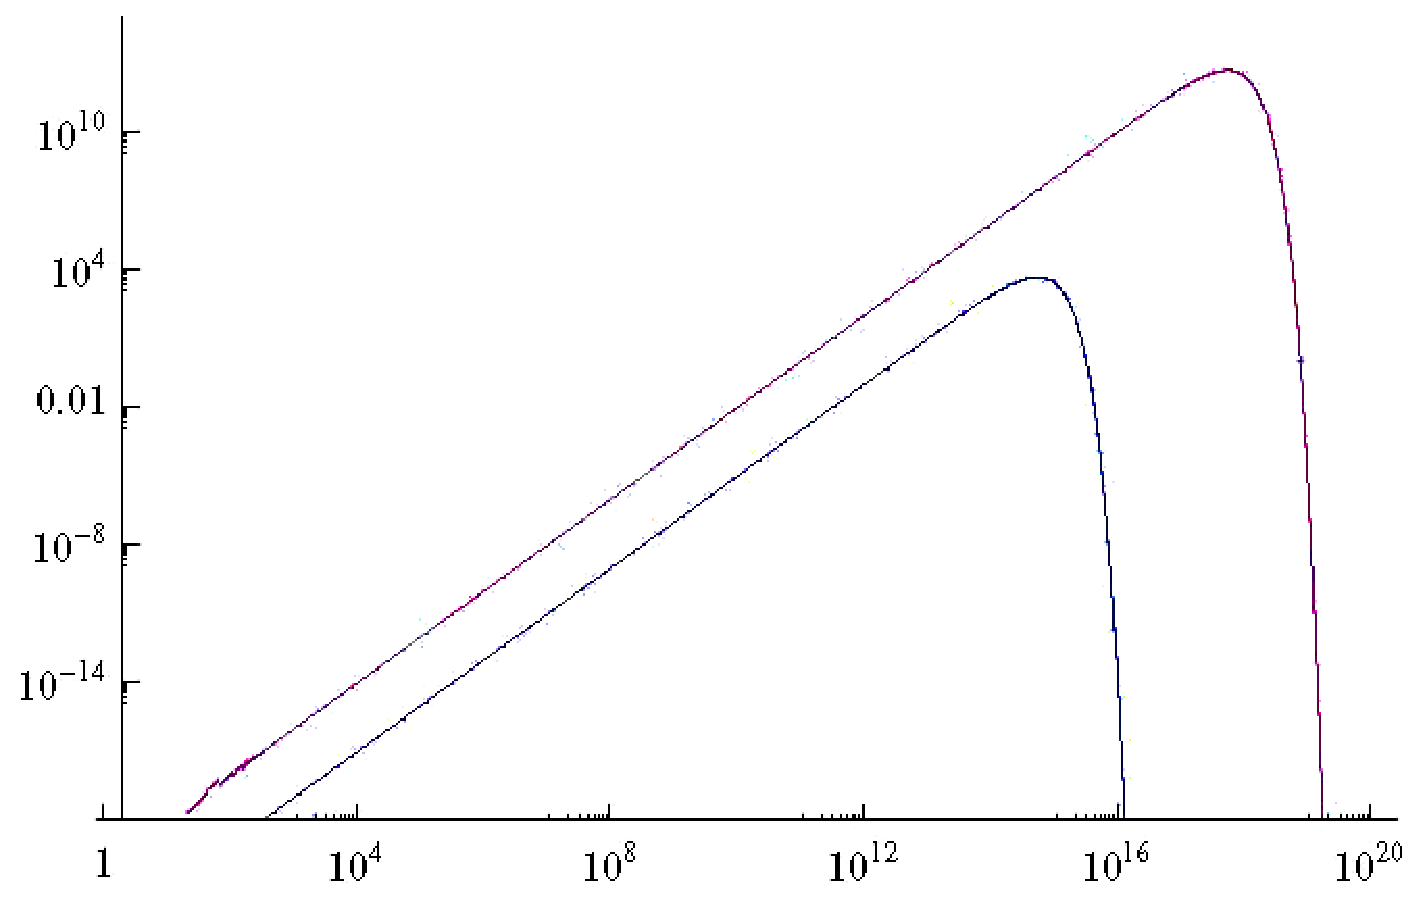
\includegraphics[width=0.6\textwidth]{2007physA6_1r.eps}\\図1
  \end{center}
\item
  \begin{align}
    F(T) &= \int\Omega\int_0^\infty \d\nu I_\nu(T)
  \end{align}
  だから,
  \begin{align}
    F(T) &= \frac{8\pi h}{c^2} \int_0^\infty \d\nu \frac{\nu^3}{\exp(\frac{h\nu}{\kB T})-1}.
  \end{align}
  ここで $p=\frac{h\nu}{\kB T}$ の変数変換をすると
  \begin{align}
    F(T) &= \frac{8\pi\kB^4T^4}{c^2h^3} \int_0^\infty \d{p} \frac{p}{e^p-1} \propto T^4.
  \end{align}
\item\ilabel{A6.5}
  もっとも遠心力が強いのは天体の表面であるから, 重力, 遠心力をそれぞれ $f_\mathrm{g},\,f_\mathrm{c}$とおくと
  \begin{align}
    f_\mathrm{g} &= G\frac{m}{R^2}\times\frac{4\pi R^3\rho}3,\\
    f_\mathrm{c} &= mR\omega^2 = \frac{4\pi^2mR}{P^2}.
  \end{align}
  ここで条件は $f_\mathrm{c}\le f_\mathrm{g}$ だから
  \begin{align}
    \rho \ge \frac{3\pi}{GP^2}
  \end{align}
  より $\rho$ の下限値は $\frac{3\pi}{GP^2}$ である.
\item
  地球から見た天体は円に見える. このことを利用し, 天体の温度を $T$, 天体までの距離を$r$,
  天体の半径を $R$ とすると
  \begin{align}
    f &\propto \frac{T^4R^2}{r^2}
  \end{align}
  となる\footnote{
  電磁波を放出している天体を中心とした球殻上で得られる単位時間あたりのエネルギーについて球殻表面で積分すると、その積分値は半
  径によらず一定になる. これがすなわち天体が単位時間に放出しているエネルギーと等しいからである. これにより地球で観測されるエネル
  ギーに関して $f\propto \frac1{r^2}$が成り立つのである.}.
  太陽の値を添え字 s で表すとすると比例関係より
  \begin{align}
    R^2 &=\frac{f}{f_\mathrm{s}}\times\left(\frac{r}{r_\mathrm{s}}\right)^2\times\left(\frac{T_\mathrm{s}}{T}\right)^4\times R_\mathrm{s}^2
  \end{align}
  となる. 与えられた数値を代入して
  \begin{align}
    R \sim 1.3\times10^4\sim 1\times 10^4[\mathrm{m}]
  \end{align}
  となる.
\item
  設問\iref{A6.5}で求めた式に数値を代入して
  \begin{align}
    \rho &= \sqrt{3\pi} GP^2 \sim 1.3\times 10^{17} \sim 1\times 10^{17} [\mathrm{kg/m^3}].
  \end{align}
  ここで水の密度は
  \begin{align}
    1[\mathrm{g/cm^3}]=10^{-3}\times 10^6 [\mathrm{kg/m^3}] = 10^3[\mathrm{kg/m^3}].
  \end{align}
  また原子核の密度は $0.17[\mathrm{核子/fm^3}]$ だから $3\times10^{17}[\mathrm{kg/m^3}]$ である.
  よってこの天体の密度は原子核のオーダーである. 天体の質量の下限を求めると,
  \begin{align}
    M = \rho\times\frac 43 \pi R^3 = 1.09\times10^{30}[\mathrm{kg}] \sim 0.5M_\odot
  \end{align}
  となる\footnote{これは中性子星と考えられる. 密度が原子核級ってことで中性子星か白色矮星が候補に挙がるが、
  中性子星の半径は 10[km] 程度, 白色矮星の半径が地球と同程度なのでこの場合は中性子星である.
  ちなみに太陽質量の 1.5$\sim$2.5 倍が限界質量で, それを超えるとブラックホールになってしまうっぽいです.
  そもそも問題の条件の表面温度が1000万度って条件から中性子星を思い浮かべると計算結果の確かめが楽
  かもしれません.}.
  %% \begin{align}
  %% \end{align}
\end{enumerate}
\end{answer}
